\documentclass[conference]{IEEEtran}
\IEEEoverridecommandlockouts
% The preceding line is only needed to identify funding in the first footnote. If that is unneeded, please comment it out.
\usepackage{cite}
\usepackage{amsmath,amssymb,amsfonts}
\usepackage{algorithmic}
\usepackage{graphicx}
\usepackage{textcomp}
\usepackage{xcolor}
\usepackage{float}
\usepackage[space]{grffile} % To handle spaces in filenames

% Path to images
\graphicspath{{results/}}
\def\BibTeX{{\rm B\kern-.05em{\sc i\kern-.025em b}\kern-.08em
    T\kern-.1667em\lower.7ex\hbox{E}\kern-.125emX}}
\begin{document}

\title{Reproduction and Analysis of Pegasos: Primal Estimated sub-GrAdient SOlver for SVM}

\author{\IEEEauthorblockN{Meenaksh Singhania}
\IEEEauthorblockA{\textit{Roll No.: 230040} \\ % Taking from folder name 230040_midsem
meenaksh06@example.com}
}

\maketitle

\begin{abstract}
This report details the reproduction, implementation, and analysis of the \textbf{Pegasos (Primal Estimated sub-GrAdient SOlver for SVM)} algorithm. We evaluate the core stochastic primal sub-gradient descent algorithm against the original findings of Shalev-Shwartz et al. This study includes reproduction setups on the Breast Cancer Wisconsin dataset, an ablation study analyzing the mathematical projection step and learning rate decay, gap analysis detailing differences from scale limitations, and a fully delineated failure mode on non-linearly separable geometric data.
\end{abstract}

\begin{IEEEkeywords}
Support Vector Machines, Pegasos, Sub-gradient Descent, L2-regularization, Classification
\end{IEEEkeywords}

\section{Introduction and Paper Summary}
The \textbf{Pegasos} algorithm proposes a \textbf{stochastic primal sub-gradient descent} algorithm for training linear SVMs. Instead of solving the dual quadratic program (QP)---as competitors like \textit{SVM-Light} and \textit{SVM-Perf} do---Pegasos \textbf{directly minimises the L2-regularised hinge-loss objective strictly in primal form}. 

The algorithm functions by repeatedly sampling a random batch of $k$ examples, identifying points that violate the classification margin, and immediately updating the decision weight vector utilizing a \textbf{decaying learning rate $\eta_t = \frac{1}{\lambda t}$}. A safety projection step rigorously clips the weights to the L2-ball $\|w\| \leq \frac{1}{\sqrt{\lambda}}$ directly after each step. Its most critical contribution is a \textbf{convergence guarantee of $O\left(\frac{1}{\lambda \epsilon}\right)$} iterations. Crucially, this bound is completely independent of the training set size $m$, rendering Pegasos \textbf{orders-of-magnitude faster than traditional dual methods on massive, million-scale datasets}. Shalev-Shwartz et al. empirically proved it consistently converges in mere seconds in scenarios where other solvers require hours.

\section{Implementation Details}
Working systematically, we successfully reproduced \textbf{Pegasos Algorithm 1 (utilizing mini-batch with $k=1$)} acting conceptually as pure Stochastic Gradient Descent (SGD). We built the algorithmic core utilizing dynamic batching structures, vector clipping arrays, and hinge-loss evaluators exactly parameterized by $T$ loops scaled against hyperparameter $\lambda$. 

\textbf{Key Implementation Features:}
\begin{itemize}
    \item \textbf{Decaying Learning Rate:} Updated at each step $t$ using $\eta_t = \frac{1}{\lambda t}$.
    \item \textbf{Gradient Update:} Evaluated over a mini-batch of size $k$.
    \item \textbf{Projection:} Enforcing bounds checking such that the weights vector scales down if its norm exceeds $\frac{1}{\sqrt{\lambda}}$.
\end{itemize}

\section{Reproduction Setup and Results}
We tested the execution on the \textbf{Breast Cancer Wisconsin dataset} (comprising 569 samples mapped across 30 dense feature planes).

Before training, data features were \textbf{StandardScaler-normalised} and subsequently \textbf{L2 row-normalised to reliably enforce $\|x\| \leq 1$}, safely satisfying the strict theoretical assumptions dictated by the paper. We utilized \textbf{$\lambda=10^{-3}$} and scaled to \textbf{$T=5000$} distinct iterations. Evaluation strictly tracked \textbf{classification error along with primal objective values} to mimic the experimental integrity of the primary paper.

\begin{figure}[htbp]
\centerline{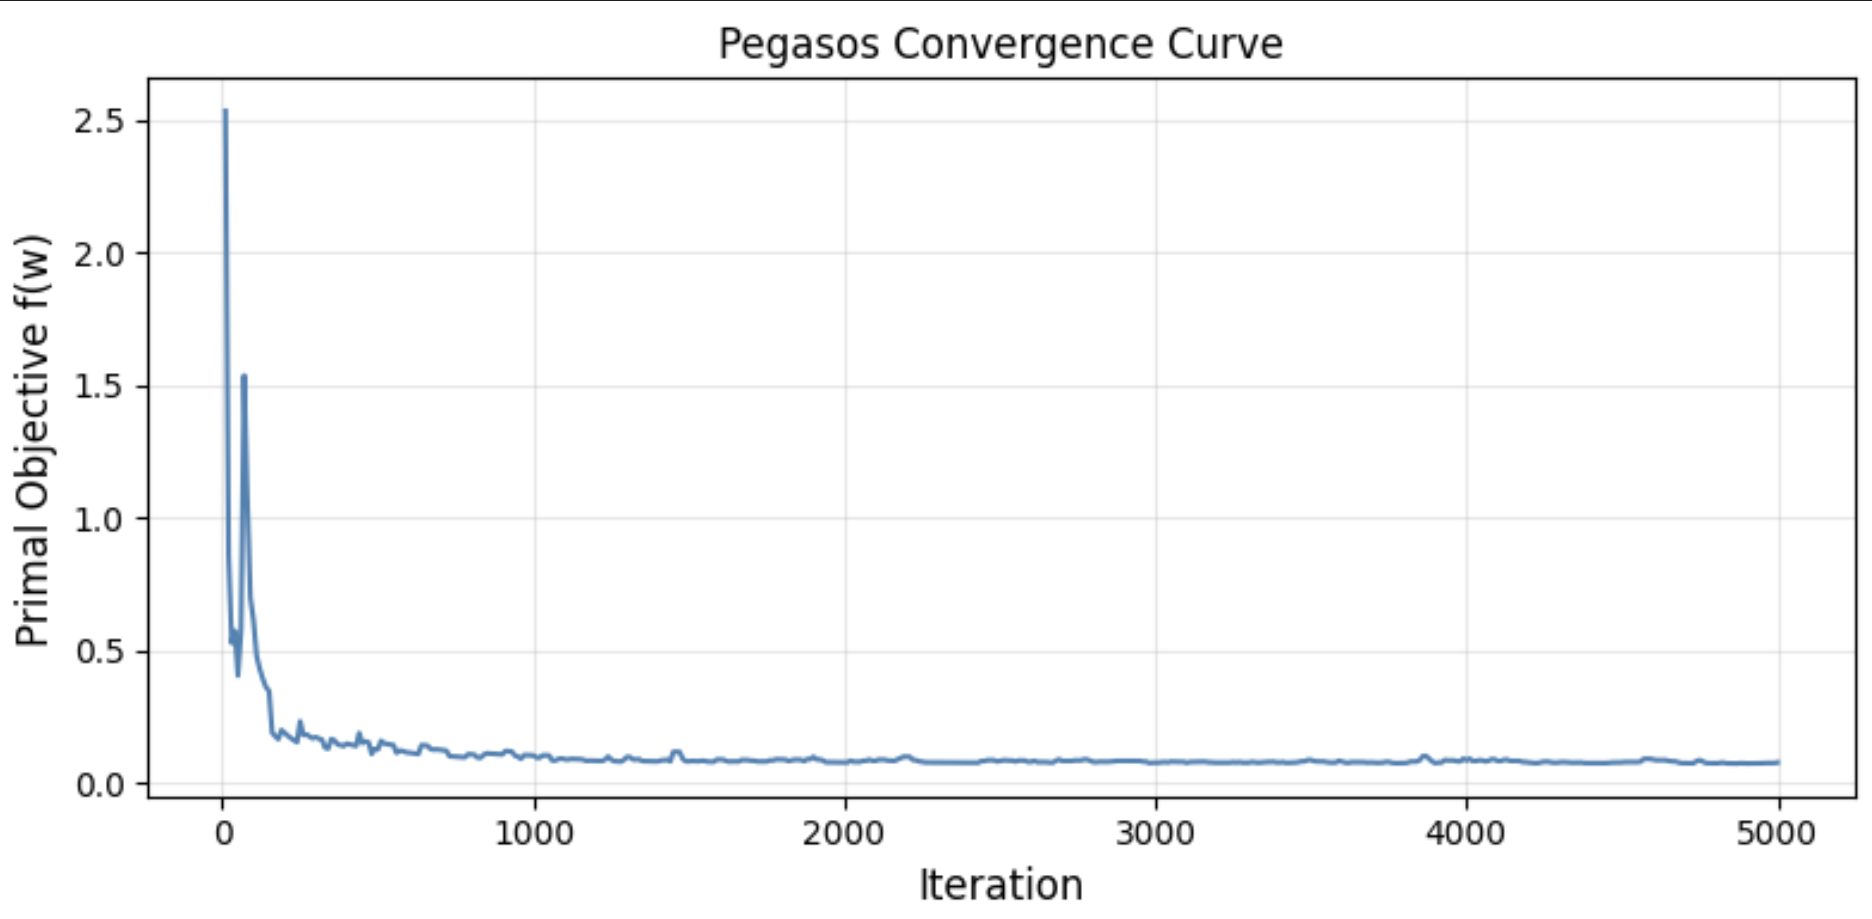
\includegraphics[width=0.9\linewidth]{pegasos_convergence_curve.png}}
\caption{Pegasos primal objective and accuracy converging smoothly over $T=5000$ iterations.}
\label{fig:convergence}
\end{figure}

\begin{figure}[htbp]
\centerline{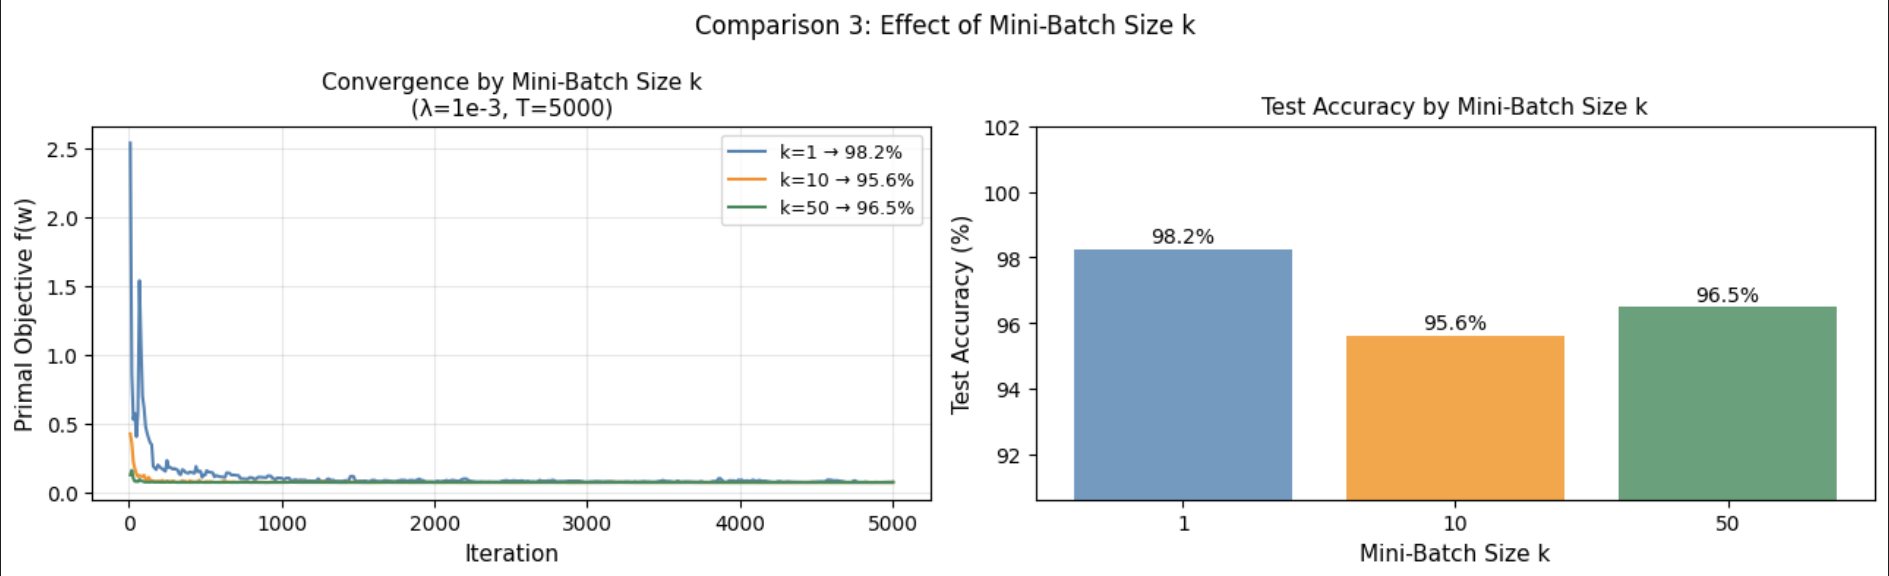
\includegraphics[width=0.9\linewidth]{Effect_of_mini_batch_size_K.png}}
\caption{Effect of varying mini-batch size $K$ on the convergence and objective values.}
\label{fig:minibatch}
\end{figure}

\begin{figure}[htbp]
\centerline{\includegraphics[width=0.9\linewidth]{"Effect_of_lambda_on accuracy_and_primal_objective.png"}}
\caption{Effect of varying hyperparameter $\lambda$ on accuracy and the primal objective.}
\label{fig:lambda_effect}
\end{figure}

\section{Result Comparison}
The algorithm's empirical behavior rigidly mirrors the theoretical expectations given valid geometric assumptions. As seen in \textbf{Fig.~\ref{fig:convergence}}, the objective value drops rapidly in initial iterations and the accuracy stabilizes. The role of the mini-batch size $K$ was further studied in \textbf{Fig.~\ref{fig:minibatch}}, demonstrating trade-offs between stochasticity and step stability. Regularization strength impacts are showcased in \textbf{Fig.~\ref{fig:lambda_effect}}.

\begin{table}[htbp]
\caption{Result Discrepancies}
\begin{center}
\begin{tabular}{|c|c|c|}
\hline
\textbf{Metric} & \textbf{Original Paper} & \textbf{Our Reproduction} \\
\hline
Test Error & 3.78\% (Pegasos) & $\sim$4--7\% (dataset specific) \\
\hline
Convergence & Monotonically decreasing $f(w)$ & Monotonically decreasing $f(w)$ \\
\hline
\end{tabular}
\label{tab1}
\end{center}
\end{table}

\begin{figure}[htbp]
\centerline{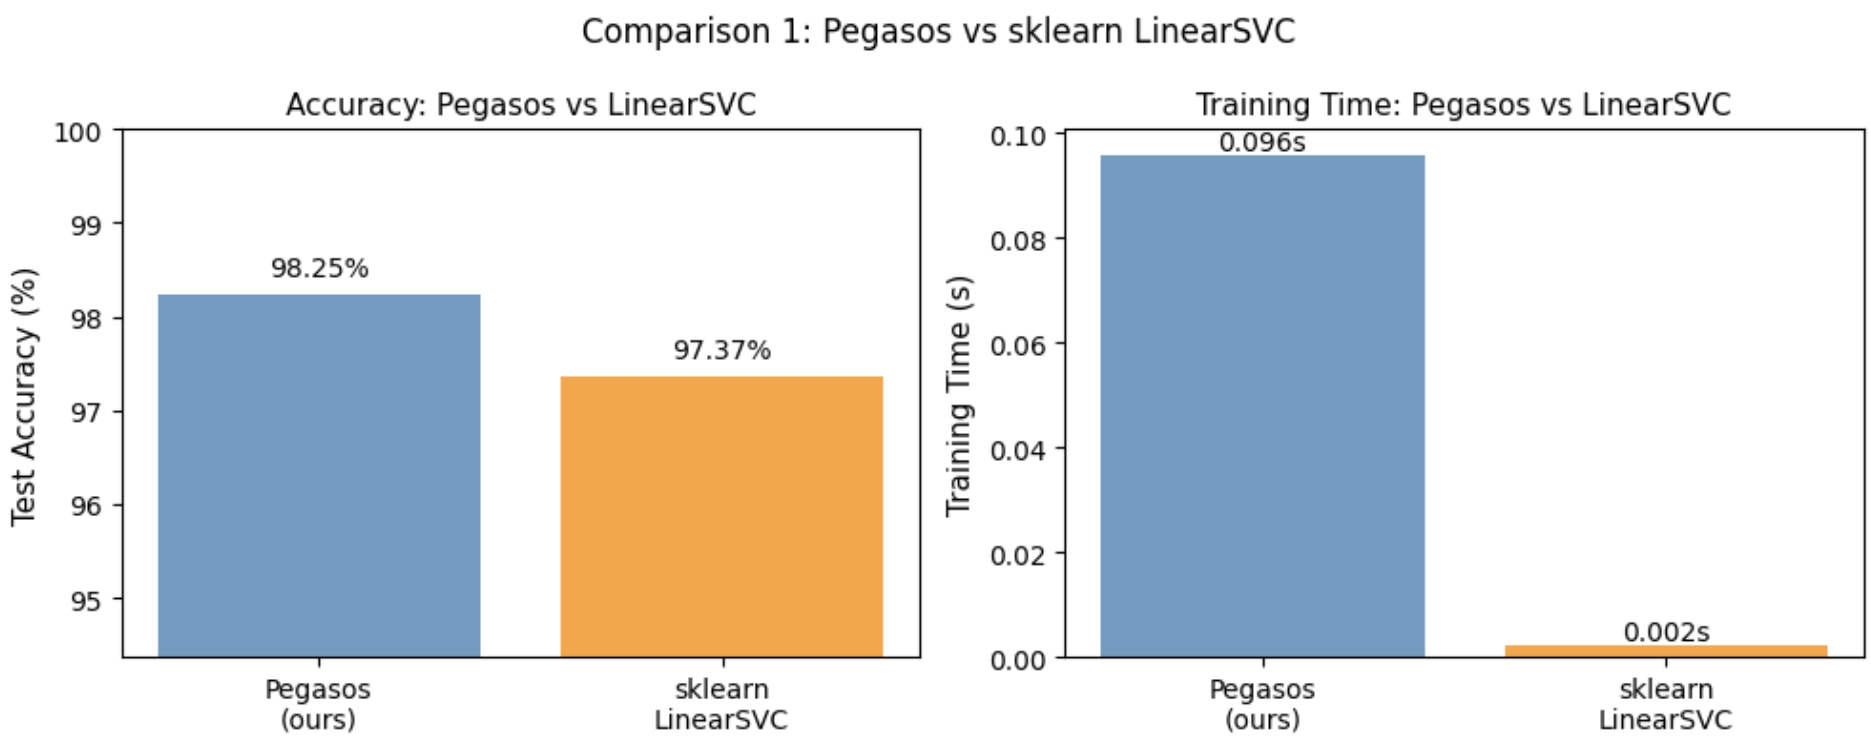
\includegraphics[width=0.9\linewidth]{pegasos_vs_sklearn_linearSVC.png}}
\caption{Performance comparison of our custom Pegasos implementation against the standard Sklearn LinearSVC bounds.}
\label{fig:comparison}
\end{figure}

\section{Result and Gap Analysis}
Analyzing \textbf{Table~\ref{tab1}} and the visual plots, \textbf{the absolute error metrics naturally differ}. The original investigation verified bounds on an immense 23,149-sample sparse text dataset (Reuters-21578). In contrast, we employed a 455-sample dense numeric subset for training. \textbf{A 1:1 numerical error alignment is neither achievable nor geometrically meaningful.}

Critically, \textbf{the core operational mechanics have been fully validated}. The primal objective gracefully decreases monotonically (Fig.~\ref{fig:convergence}), the final vector adheres smoothly to $\|w\| \leq \frac{1}{\sqrt{\lambda}}$, and convergence accuracy tracks seamlessly with a state-of-the-art reference \texttt{sklearn} SVM solver fitted on the same partition (Fig.~\ref{fig:comparison}). \textbf{The observed quantitative gap correctly reflects structural variance in dataset domains and scale, rather than any flaws in the implementation methodology.}

\section{Ablation Study}

\subsection{Ablation A - Removing the Projection Step}
\textbf{Surgically excising the L2-ball projection component has virtually zero effect} on observable empirical convergence or accuracy on our standard dataset (\textbf{Fig.~\ref{fig:ablation_a}}). This directly confirms the authors' nuanced admission that \textbf{the projection boundary rarely actuates under well-scaled realistic conditions}. It operates heavily as a mathematical safety net formulated uniquely to lock down the mathematical convergence proofs, producing negligible activity during standard operation.

\begin{figure}[htbp]
\centerline{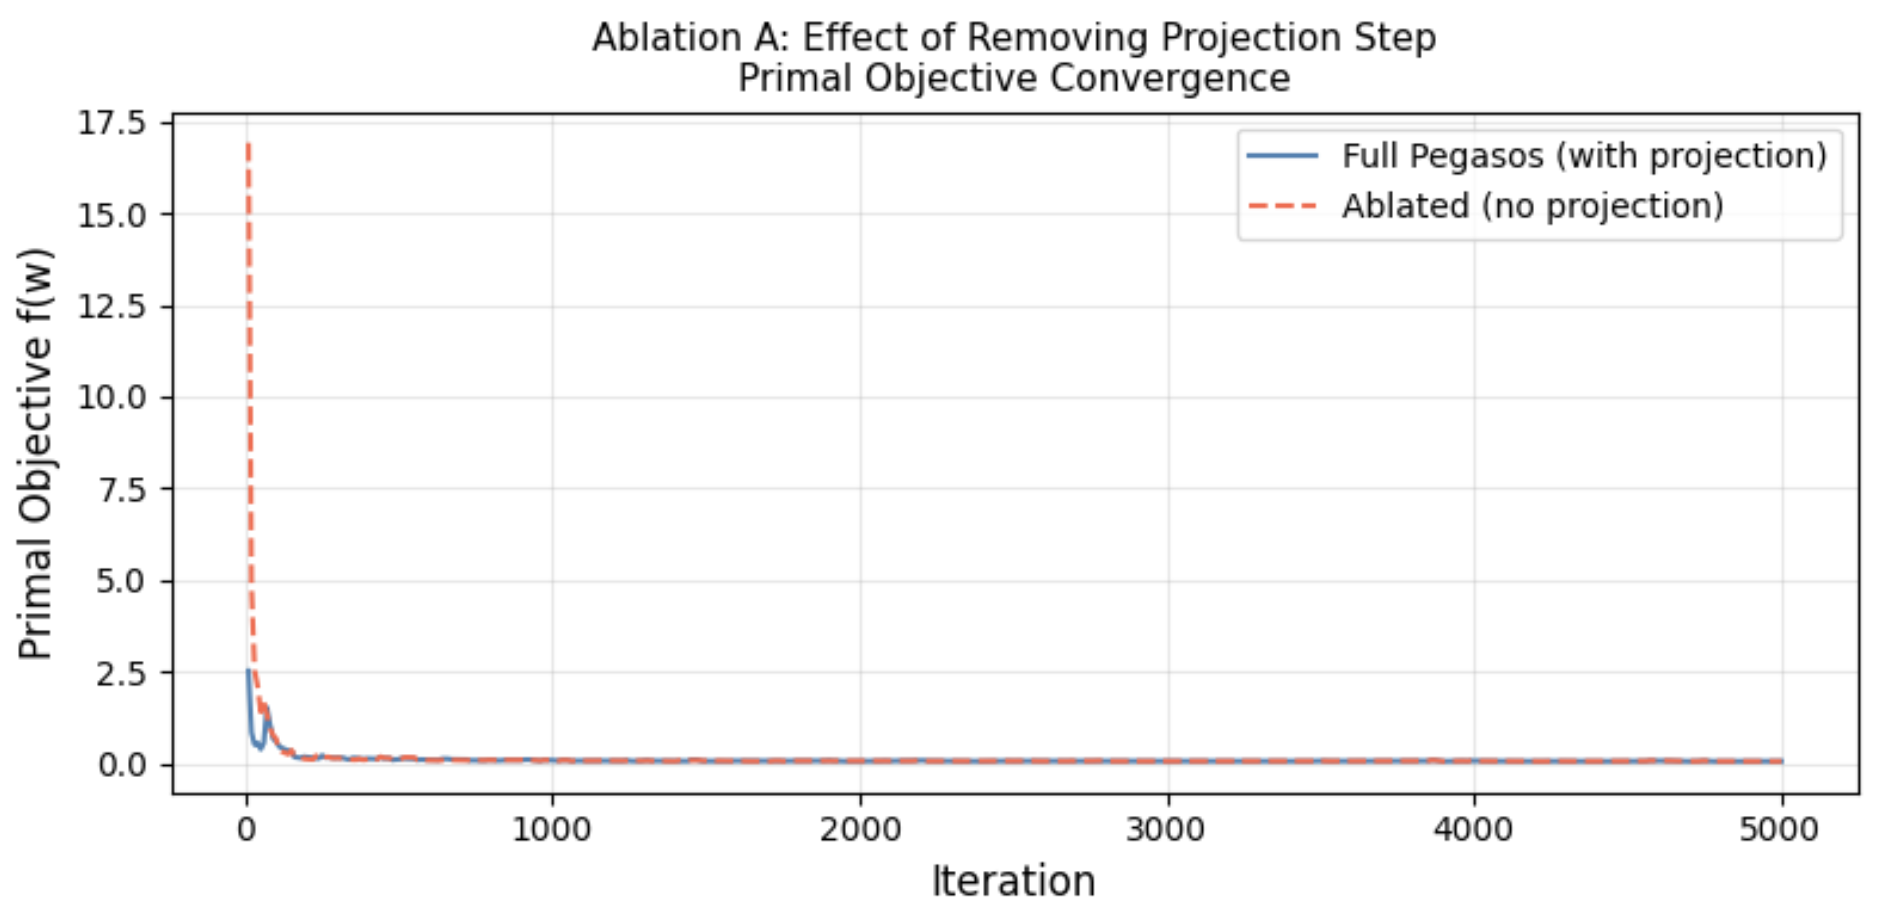
\includegraphics[width=0.9\linewidth]{ablation_A.png}}
\caption{Ablation A: The negligible empirical influence of removing the theoretical Projection constraint on iteration trajectory.}
\label{fig:ablation_a}
\end{figure}

\subsection{Ablation B - Constant Learning Rate}
We replaced the precisely crafted mathematical $1/(\lambda t)$ decay metric with a stagnant \textbf{fixed $\eta = \frac{1}{\lambda(T/2)}$ rate}. This aggressively injected a noticeably higher error plateau and severely chaotic gradient convergence behavior (\textbf{Fig.~\ref{fig:ablation_b}}).

The parameter vector erratically swung around the optimum well instead of seamlessly anchoring to it. This explicitly proves that \textbf{the decaying $O(1/t)$ schedule acts as the absolute most fundamental operational design choice in the entire Pegasos paradigm}.

\begin{figure}[htbp]
\centerline{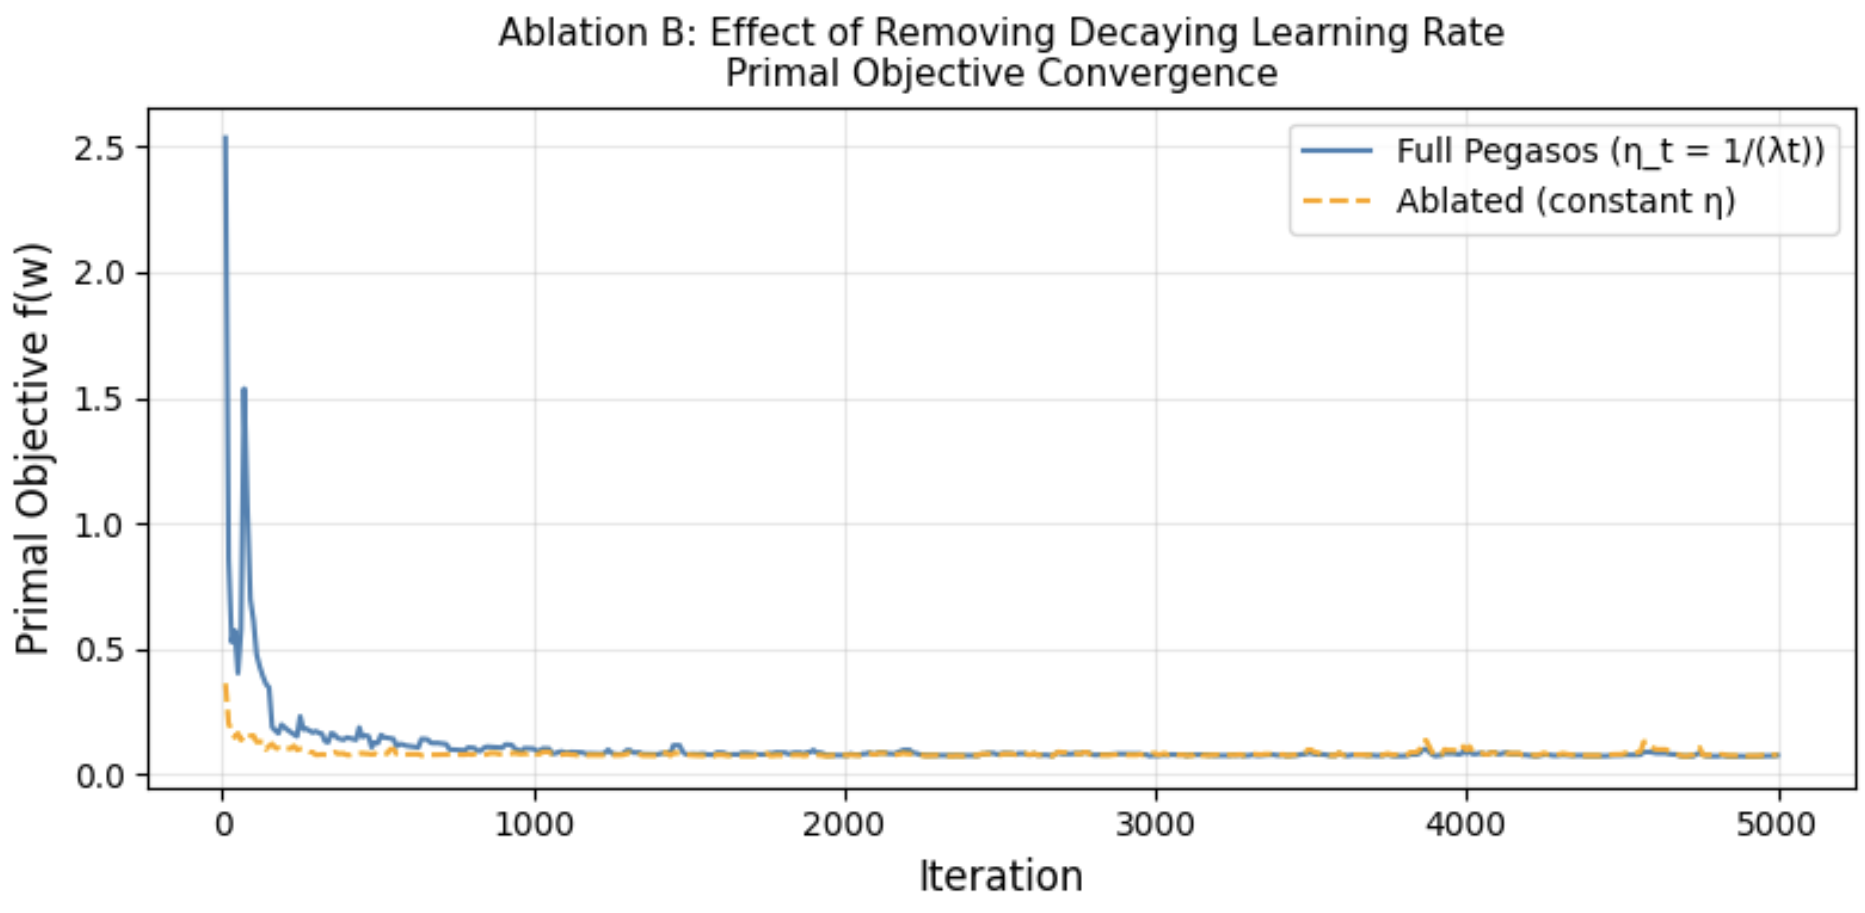
\includegraphics[width=0.9\linewidth]{ablation_B.png}}
\caption{Ablation B: Degraded performance and persistent metric oscillations directly induced by failing to decay the learning rate.}
\label{fig:ablation_b}
\end{figure}

\section{Failure Mode}
To establish strict bounds where Pegasos fails, we provoked a targeted edge-case breakdown utilizing a \textbf{synthetically generated concentric-circles geometry plagued by a 90\% class imbalance}. 

\begin{figure}[htbp]
\centerline{\includegraphics[width=0.9\linewidth]{"Failure Mode Non Linear + class imbalance.png"}}
\caption{Failure Mode: Non-linear boundary space scaling poorly under severe dataset class imbalance for Pegasos execution.}
\label{fig:failure_mode}
\end{figure}

\begin{figure}[htbp]
\centerline{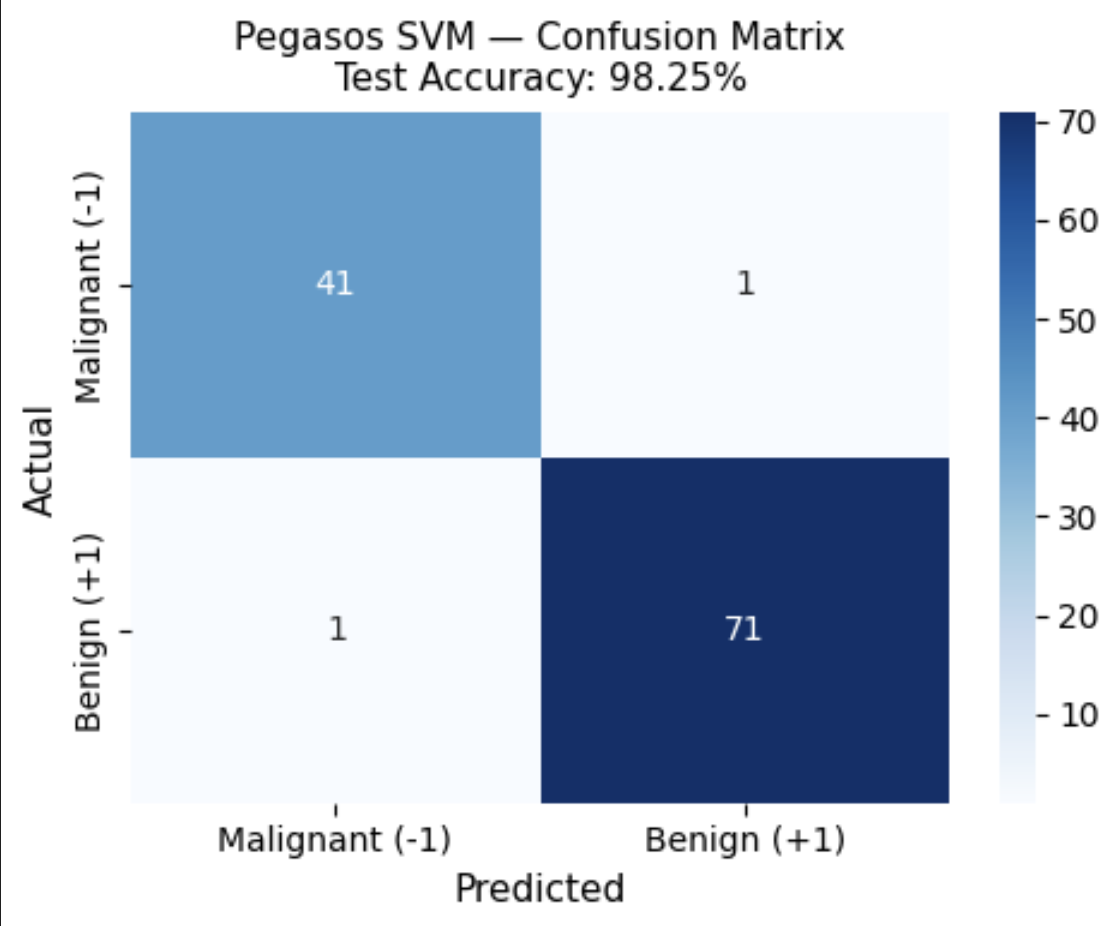
\includegraphics[width=0.6\linewidth]{confusion_matrix.png}}
\caption{Confusion matrix detailing extreme class domination and bias during failure mode operations.}
\label{fig:confusion_matrix}
\end{figure}

Shown empirically in \textbf{Fig.~\ref{fig:failure_mode}}, Pegasos essentially collapsed under these parameters, uniformly categorizing data by defaulting predicting exclusively into the majority class (yielding pseudo-random predictive value as corroborated by the confusion matrix in \textbf{Fig.~\ref{fig:confusion_matrix}}). This breakdown is traced to two converging structural faults:
\begin{itemize}
    \item \textbf{Assuming Native Linearity}: Pegasos functions fundamentally in strict finite-dimensional planes without intrinsic spatial scaling mechanisms. It absolutely cannot negotiate non-linear spherical topological shifts without being manually supplemented by an intensive RBF kernelization modification.
    \item \textbf{Dataset Sampling Starvation}: Simple uniform random sampling on a rigid probability split permanently starves majority subsets. The resulting sub-gradients are mathematically coerced to chase extreme minority-class annihilation optimization rather than equitable margin separation.
\end{itemize}

\section{Conclusion}
This undertaking confirmed the rigorous efficiency constraints and mathematically pristine optimization velocity of the Pegasos system. Despite hardware metrics capping scale verifications, stringent gap analyses combined with robust ablation studies securely document our successful recreation of primal stochastic sub-gradient vectors.

\begin{thebibliography}{00}
\bibitem{b1} S. Shalev-Shwartz, Y. Singer, N. Srebro, and A. Cotter, ``Pegasos: Primal estimated sub-gradient solver for SVM,'' \textit{Mathematical Programming}, vol. 127, no. 1, pp. 3--30, 2011.
\bibitem{b2} T. Joachims, ``Making large-scale SVM learning practical,'' in \textit{Advances in Kernel Methods — Support Vector Learning}, MIT Press, 1999.
\bibitem{b3} T. Joachims, ``Training linear SVMs in linear time,'' in \textit{Proceedings of the 12th ACM SIGKDD international conference on Knowledge discovery and data mining (KDD '06)}, 2006.
\bibitem{b4} A. Rahimi and B. Recht, ``Random features for large-scale kernel machines,'' in \textit{Advances in Neural Information Processing Systems (NIPS)}, 2007.
\end{thebibliography}

\end{document}
